%%
%% 第三章
%% 2012.5.22


\chapter{大规模近似重复图像搜索算法概述}

随着多媒体业务的日益增长,近似重复图像搜索(Near Duplicate Image Retrieval)或部分重复图像搜索(Partial Duplicate Image Retrieval)技术得到了愈加广泛的应用。在我们的图像重建系统中的相似图像搜索环节,我们希望找到尽可能多的与用户拍摄图像相似的图像,将其作为后续重建环节的候选图像。因此我们面临的三个技术难点是:(1)相似搜索是在图像的局部进行的,而不是整幅图像,所以使用全局特征进行相似图像搜索的传统方案并不适用,是否有能表述局部特性的图像表示方法;(2)图像的局部特征信息较少,如何充分利用特征之间的几何位置关系进行图像局部匹配来提高搜索精度;(3)云端图像数据库是Web规模的(Web-Scale),图像数据量极大,对算法的时空复杂度限制较大。如何在使用图像局部特征和其空间位置关系的同时尽量不增加搜索算法的复杂度,是本系统需要解决的难题。

本章首先介绍传统的图像搜索算法,再介绍利用局部特征的空间信息的相似图像搜索算法,最后针对本论文的应用场景,提出一种结合多种技术的新的相似图像搜索技术。

%%%%----------------------------------------相似图像搜索--------------------------------------------%%%%
\section{基于局部特征的相似图像搜索算法}

最常见的基于局部特征的相似搜索算法包含两个环节。第一步,从图像中提取局部特征,图像的感兴趣区域可以通过自动的特征点检测或者均匀取样获得,最常见的局部特征描述子包括梯度方向直方图(histograms of oriented gradient,HOG)和SIFT、SURF等。从一幅图像抽取的特征集合叫做视觉词袋(Bag of Visual Words)。在第二步中,我们需要定义两个视觉词袋之间的相似性,第一类是直接比较两个视觉词袋的相似性,例如投票方法;第二类是通过视觉词袋计算一个特征签名(signature,通常是一个向量),进而比较两个签名之间的相似度。两种方式都需要对数据库中的所有图像与请求的图像比较相似度并排序\cite{POLICY:2013te}。

\subsection{视觉词袋模型}
视觉词袋(Bag of Visual Words)模型是图像表示中最为经典的一种表示方法。它经常被用来进行图像分类和相似性搜索领域。它来自文档检索基于关键字查询的方法中词袋(Bag of Words)的表示方法,其基本思想是:(1)统计语料库中的所有单词,生成单词表;(2)对于每一篇文档,统计每一个单词出现的频次,用由这些单词出现的次数生成直方图,用直方图来表示这篇文档。这种直方图的表示就是词袋表示。视觉词袋类似于BoW模型,算法的基本思路如下:

(1)离线部分:
\begin{itemize}
\item 提取特征:根据使用场景与实际业务的不同,可以选择不同的特征,文献\cite{Zhang:2006ej}对视觉词袋模型进行深入的分析,综合比较了各种特征检测器、描述子等。在这一步,我们综合考虑特征的时空复杂度、鲁棒性、可区分性等。
\item 生成视觉词码表:统计图像数据库中出现的所有特征,去除冗余的特征(比如几乎每一篇文档中都会出现的特征,类似于文档中的停用词)组成视觉词码表(Codebook)。如果提取的图像特征过多,一般需要对特征进行量化,利用聚类算法先把相近的单词归为一类(类似于文档检索里的找词根),利用聚类的结果生成视觉词码表。
\item 利用视觉词码表量化所有的图像特征
\item 利用词频表示的词袋模型来表示数据库中的每一幅图像
\end{itemize}

(2)在线部分:
\begin{itemize}
\item 提取请求图像的局部特征;
\item 利用视觉词码表量化该图像的图像特征;
\item 利用词频表示的词袋模型来表示请求图像;
\item 利用词频表示做进一步的处理,例如分类,相似性比较等。
\end{itemize}

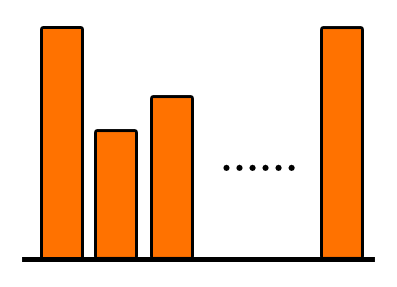
\includegraphics[width=5.00cm]{imgs/ch3/histogram}

\subsection{局部特征的聚类}
生成视觉词码表是将局部特征进行聚类的过程,最经典的聚类算法是K均值聚类(K-MEANS),在实际中,我们通常在云端图像语料集中随机的选取一部分的特征,对这部分特征使用K-MEANS进行聚类,确定所有类中心后,再对语料集中的所有特征进行处理,找到每一个特征距离最近的类中心,完成对所有局部特征的量化。后续的请求图像在提取特征后按照同样的方式进行量化。

然而,在本文提出的系统中,图像局部特征数量极大(对于上百万图像素的图像来说,每幅图像的sift数量平均在3000以上,100K的图像集上,有300M以上个128D的特征。),传统的K-MEANS不能满足我们的性能要求,最近的一些研究针对图像据图特征提出了许多快速聚类的方法,文献\cite{Philbin:2007fk,Muja:2009uv,Wang:2010vs}等提出了近似K聚类(Approximate K-MEANS,AKM)和结构化K聚类(Hierarchy K-MEANS,HKM)的方案,
。

近似K-MEANS是传统K-MEANS的一种替代,传统的K-MEANS的时间花销主要是在计算特征点最近邻的类中心上,每一次迭代,我们需要计算每一个特征点,计算它和每一个类中心的距离,所以每次迭代的时间复杂度是\(O(NK)\),其中N是特征点数量,K是类中心的数量。在改进的版本中,每一次迭代之前,我们使用随机k-d森林来构建类中心来加快速度。在常规的k-d树中,我们需要决定每一次划分是在哪一个维的哪一个点上,通常我们选择方差最大的一个维度作为划分维度,以该维度上中值点作为划分点,在同一维度上比划分点小的点落在k-d数当前节点的左侧,大的落在右侧。在随机k-d森林中,每一棵k-d树都是构建在所有的类中心上,不过在构建时采用划分策略有所不同,划分维度是方差较大的几个维度中随机选择的,划分点也是随机的在中值附近选择一个点。所有的k-d树组成了k-d森林,这个森林构建了一个互相交叠的特征划分空间。因为量化的存在,一个在划分边缘的特征很可能找到错误的最近邻类中心,而互相交叠的划分方式则大大减轻了这一影响,增强了高维计算的鲁棒性。

计算一个特征点所属类的过程如下:
对随机森林中的每一棵树,递归的下滤到其叶子节点,计算它到可区分边界的距离,将所有的距离记录在一个优先队列中。迭代的选择最近的划分,持续的将隐藏节点加入到优先级队列中,当迭代次数达到指定数值的时候,搜索停止。

K-MEANS的时间复杂度是\(O(NK+N) = O(NK)\),AKM算法的时间复杂度是\(O(Nlog(K)\)。实验表明,AKM在大幅降低时间复杂度的同时,保证了正确率(与K-MEANS划分的类中中心相比不一致的几率<1\%)。
--------------------------------------TO Do Here---------------------------

\subsection{相似性度量}
%[相似度计算](http://blog.sina.com.cn/s/blog_6634c1410100w56x.html)

%%%%----------------------------------------改进--------------------------------------------%%%%
\section{改进的相似搜索算法}
文献\cite{POLICY:2013te}对近期的大规模相似图像搜索技术做了总结,提到了Partial-Duplicate Image Retrieval via Saliency-Guided Visual Matching\cite{Li:2013ks}技术,
通过视觉显著性(saliency)模型进行比较,消除背景中的噪声。这种方法使得索引和匹配都集中在显著性区域,更能够符合用户的预期。显著值和空间约束都能够被用来进行相似性度量,并且能够高效的进行二级索引,对于大规模的partial duplicate search非常有利,但是内存开销比较大。

Web-Scale Image Retrieval Using Compact Tensor Aggregation of Visual Descriptors\cite{Negrel:2013ur}描述了目前存在的各种视觉描述子的概况,介绍了相关的索引技术,包括哈希、词袋以及基于树的表示方法。(hashing, bag-of-words, and tree-based representation)引出内存开销问题并提出一种生成高度压缩签名(highly compact signatures)的方法,包括张量聚合,PCA,kernel PCA等一些列算法。它改进了Fisher Vector族 描述子,提高它的可区分性,以及特征签名的大小(feature discrimina- tive power and the size of feature signature)。

对于相似性视频搜索,它的特点是特征维数特别大,有研究提出了稀疏投影方式进行特征降维,并且使用数据挖掘的知识使用一些metadata来共同进行搜索\cite{Wu:2013tb}。使用机器学习技术,学习稀疏投影矩阵(sparse projection matrices)。这种学习方法可以选择性的使用外部信息,比如WikiPedia上的知识和Google搜索结果中的摘要,创建一个语义相关的投影矩阵,生成一个压缩签名,以满足手机媒体检索的诸多限制。手机内存空间小,计算资源有限,传统的将高维特征映射到低维的投影矩阵在手机内存是放不下的。而我们的稀疏投影矩阵是能够在手机上使用的。

下面我们简单介绍各种性能改进的方法。

\subsection{sim-hash}
文本的去重算法中常见的有余弦夹角算法、欧式距离、Jaccard相似度、最长公共子串、编辑距离等,但是只适合于小数据集。simhash传统的用来判断两篇文章的相似度,将两篇文章映射到低维空间上,并且保持它们互相之间的相似度,但是它很难应用在图像比较上,因为图像的特征是用实数来表示的,尽管可以将其量化,但是两幅相似图像量化后的特征集合交叠的比率仍旧很小,远远小于文档,因为两幅图像不相似的区域的噪声特征非常大。但是如果使用视觉词组,那么如果两个相似区域的视觉词组会非常相同,我们就可以使用simhash了。所以,min-hash的使用场景是特征比较多,相似度比较显著的情况下。

\subsection{最小哈希的相似性比较}
最小哈希方法是一种广泛应用在相似性查找领域的算法。

在生成视觉词带之后,比较两幅图像或者两篇文章的相似度问题转化为比较两个只包含0,1元素的集合的相似度,集合的相似度是Jaccard相似度。
\[JS(A,B)=\frac{|A\cap{B}|}{|A\cup{B}|}\]
我们首先定义一组随机哈希函数\(f_j:\mathcal{V} \to R\),每一个哈希函数是独立的,将一个视觉词映射为一个实数。两个不同的视觉词\(X_a\)和\(X_b\),哈希函数需要满足两点:(1)\(f_j(X_a)\neq f_j(X_b)\);(2)\(P(f_j(X_a)) < (P(f_j(X_b)) = 0.5\)。

注意到函数\(f_j\)能够反映出视觉词集合的一个顺序排列情况,我们定义min-hash就是这个排列中排在最前面的视觉词,因此有
\[m(\mathcal{A}_i,f_j)= arg\mathop {\min }\limits_{X \in A_i}f_j(X)\]
根据上述定义,我们会发现以下这个事实:
\[Pr(m(A,f_j) = (B,f_j)) = \frac{|A\cap{B}|}{|A\cup{B}|} = sim_s(A,B)\]

如果r是随机变量,当\(m(A,f_j) = (B,f_j)\)时值为1,其它情况下值为0的,那么r可认为是J(A,B)的无偏估计。因此我们可以使用min-hash函数将一幅图片或者一篇文章转化为一个数(对该文章中的每一个单词id使用hash函数后得到一个新的id序列,这个序列中的第一个出现1的行号,就是min-hash的值),当我们使用k个hash函数,得到k个值,将原本的高维向量映射到了低维。min-hash在压缩原始集合的情况下,保证了集合的相似度没有被破坏。
文献\cite{Chum:2008jo}中提出将词频-逆文档频率(term frequency–inverse document frequency,简称TF-IDF)融合在传统的min-hash算法中,实验表明能够提高搜索的准确率。

\subsection{LSH}
使用min-hash对数据降维后,可以使用LSH缩小查找范围,其基本思路是将相似的集合聚集到一起,减小查找范围,避免比较不相似的集合。

对每一列c(即每个集合)我们都计算出了n行min-hash值,我们把这n个值均分成b组,每组包含相邻的r=n/b行。对于每一列,把其每组的r个数都算一个hash值出来,把此列的编号记录到hash值对应的bucket里。如果两列被放到了同一个bucket里,说明它们至少有一组(r个)数的hash值相同,此时可认为它们有较大可能相似度较高(称为一对candidate)。最后在比较时只对落在同一个bucket里的集合两两计算,而不是全部的两两比较。

%%%%----------------------------------------空间信息匹配搜索算法--------------------------------------------%%%%

\section{基于空间信息的匹配搜索算法}
使用视觉词袋模型来表示图像并比较视觉词袋之间的相似性做法比较成熟、最为普及的做法
\subsection{随机抽样一致算法}
随机抽样一致RANdom SAmple Consensus(RANSAC)是一种空间匹配算法。该算法将数据分成两类,局内点(inlier)和局外点(outlier)它可以从一组包含局外点的观测数据集中,通过迭代方式估计数学模型的参数。

这是一种不确定的算法,有一定的概率得出一个正确的或者说是可接受的合理结果;一般情况下,迭代次数的增加可以提升结果的准确性。该算法由Fischler和Bolles于1981年提出,在图像检索中,RANSAC可以作为检索后的后续处理,对图像的中目标进行空间一致验证。

RANSAC算法对数据集做了三个假设:

\begin{itemize}
\item 数据由局内点组成,局内点的数据的分布符合某一特定的概率模型;
\item 与局内点相对的是局外点,他们不能够适应该模型;
\item 局内点与局外点之外的数据属于噪声
\end{itemize}

RANSAC有以下几个步骤:
\begin{itemize}
\item 随机选择数据集合的一个子集
\item 使用选择的自己拟合一个数学模型
\item 确定该模型下局外点的个数
\item 重复步骤1~3若干次,以最好的一次结果最为最终拟合出来的数学模型
\end{itemize}

RANSAC算法迭代次数的选取取决于我们期望的准确率与样本数量。设p为任意给定对应点合法的概率,即
\[p = \frac{\text{局内点的数量}}{\text{数据集全部数据的数量}}\]
而P是经过S次试验后成功的总体概率。设我们需要k个随机样本来估计模型,那么在一次试验中,该k个样本都是局内点的可能性为\(p^k\)。因此,S次试验失败的可能性是
\[1 - P = (1 - p^k)^S\]
两边去对数,得到最少需要的试验次数是
\[S = \frac{log(1-P)}{log(1-p^k)}\]
随着k的增大,需要的最少试验次数增多,在实际中,我们应该尽可能的选择小的k值。在模型确定以及最大迭代次数允许的情况下,RANSAC总是能找到最优解。对于含有较大误差的数据集,RANSAC的效果远优于直接的最小二乘法。 

当对两幅图像进行匹配的时候,所以相互匹配的局部特征作为数据全集,我们要估算的模型是一个变换矩阵H,能够将图像\(I\)投影到图像\(I'\)。每次迭代过程中,随机的选择四对匹配的特征点,根据这四个特征点的位置信息解得变换H,利用H计算其它匹配对的位置信息中有哪些属于局外点,记录局外点的个数。局外点的个数越少,变换矩阵H越准确。反复迭代多次得到一个相对准确的透视变换模型。

上述提到的用四对匹配点拟合出的变换矩阵叫做单应矩阵(Homography),最简单的求解单应性矩阵的算法叫做直接线性变换法(Direct Linear Transform,DLT)\cite{Dubrofsky:2009tz},其具体算法如下:

假设我们相匹配的一对点分别是\(x\)和\(x'\),单应性矩阵是\(H\),那么有如下等式:

\begin{equation}
\label{homography1}
	c
	\begin{pmatrix}
	u \\
	v \\
	1
	\end{pmatrix}
	= H
	\begin{pmatrix}
	x \\
	y \\
	1
	\end{pmatrix}
\end{equation}


其中c是一个非零常数,\((u\ v\ 1)^\mathrm{T}\)代表\(x'\),\((x \ y \ 1)^\mathrm{T}\)代表\(x\),而
\(
H = 
\begin{pmatrix}
h_1 & h_2 & h_3 \\
h_4 & h_5 & h_6 \\
h_7 & h_8 & h_9
\end{pmatrix}
\)

将公式\eqref{homography1}展开,分别用第一行和第二行除以第三行,得到

\begin{equation}
\label{homography2}
-h_1x - h_2y - h_3 + (h_7x+h_8y+h_9)u = 0
\end{equation}

\begin{equation}
\label{homography3}
-h_4x - h_5y - h_6 + (h_7x+h_8y+h_9)u = 0
\end{equation}

公式\eqref{homography2}和\eqref{homography3}可以写成矩阵的形式:
\begin{equation}
\label{homography4}
A_ih = 0
\end{equation}

其中
\(A_i = 
\begin{pmatrix}
-x & -y & -1 & 0 & 0 & 0 &ux & uy & u \\
0 & 0 & 0 & -x & -y & -1 &vx & vy & v 
\end{pmatrix}\)
,而
\(h = (h_1 \ \ h_2 \ \ h_3 \ \ h_4 \ \ h_5 \ \ h_6 \ \ h_7 \ \ h_8 \ \ h_9)^\mathrm{T}\)。
因为每一对匹配的点可以提供两个等式,对于解决8自由度的矩阵H,只需要四对(任意三点不能共线)匹配的特征点。

DLT算法依赖于坐标系的原点和尺度,所以该算法并不稳定,在实际中更多的使用多个匹配点得到更多的方程,将求单应矩阵的问题转化为求解最小二乘的问题,用矩阵奇异值分解(Singular value decomposition,SVD)的方法来求解等式\(Ah = 0\)。

\subsection{视觉词组}

图像搜索与文本搜索的一个显著区别是图像是二维的,包含大量的空间关系信息,而BoW的一个被人诟病的问题便是没有利用任何的图像空间信息。随着图像业务需求的提高,有更多的学者提出利用图像局部特征的空间位置信息进行更加精确的相似图像搜索\cite{Philbin:2007fk,Wu:2009bl,Zhou:2010tv,Zhou:2013jz,Xu:2013wc}。

文献\cite{Xu:2013wc}深入研究SIFT描述子。提出了一个非常优雅的方法:生成SIFT组,嵌入几何信息,最终将一组SIFT压缩到一个64比特的二维签名中,叫做Nested-SIFT。它的优点是Nested—SIFT使用SIFT描述子的嵌套关系,很自然的将不同尺度的局部关键点组合在一起,生成一个特征签名。嵌入空间信息的Nested—SIFT可区分性更强。使用SimHash进行压缩后,在视觉搜索中效率更高。实验结果表明这种方法提高搜索的准确度,减少了内存消耗,提高搜索速度。其缺点是生成Nested-SIFT会有一定的计算消耗。

文献\cite{Zhou:2013jz}采用较为复杂的空间编码,对图像2D空间进行了不同维度的划分,区分了局部特征的水平与垂直方向,并且加入了扇形区域的编码,增加了视觉词组的旋转不变性。该算法较为复杂,适用于全局图像的相似查询,实验结果表明加入空间信息验证后,能够提升准确率,两幅不相关的图像可能会有相似的特征集合,但是相似特征集合在空间位置上依然保持相似的概率极低。

因为本文系统需要查询的是具有局部相似的图像块,相比于其他相似性匹配算法,我们需要的图像块粒度更细,即云端图像与请求图像全局相似度可能很低,但是局部相似度非常高,这幅图像也会被加入到候选图像中。文献\cite{Dai:2012vn}提出了简洁的做法将一个图像块内的局部特征编码成视觉词组。本位在该文基础上稍作改进,在保证算法效率的同时,增加了对算子尺度的编码,进一步增强其准确度。

对于每一个图像块而言,中心位置有一个视觉词,该视觉词的尺度与其覆盖范围(影响范围)成正比,在该范围内,有若干视觉词,我们将范围内的所有视觉词看做一个视觉词组(Visual Words Group)。我们希望将词组内的每一个视觉词分配一个编码x,表征这个词在视觉词组的相对关系,这样我们可以采用如下的规则进行匹配:
\begin{equation}
E_m(G_x,G_y) = E_v(G_x,G_y) - E_r(G_x,G_y)
\end{equation}
其中\(E_v(G_x,G_y)\)是能够匹配上的视觉词,这里匹配上定义为两个视觉词相同,并且含有相同的编码x。其中\(E_r(G_x,G_y)\)是错误匹配的视觉词,错误匹配是指两个视觉词相同,但是含有不同的编码x。

那么怎样编码视觉词,能够体现视觉词的相对关系呢?我们从两个维度对视觉词进行编码,一个是它与中心视觉词的相对方向,另一个是相对尺度大小。视觉词组的中心词的主方向作为基准方向,沿着顺时针或者逆时针方向,将整个区域分成n个子区域。接下来对于每一个子区域,根据sift算子量化前的尺度信息对比值大小的不同,将子区域分成r个维度,这样一个视觉词共有n*r个子区域,如图\ref{fig:visual_group}所示。

\begin{figure}
\centering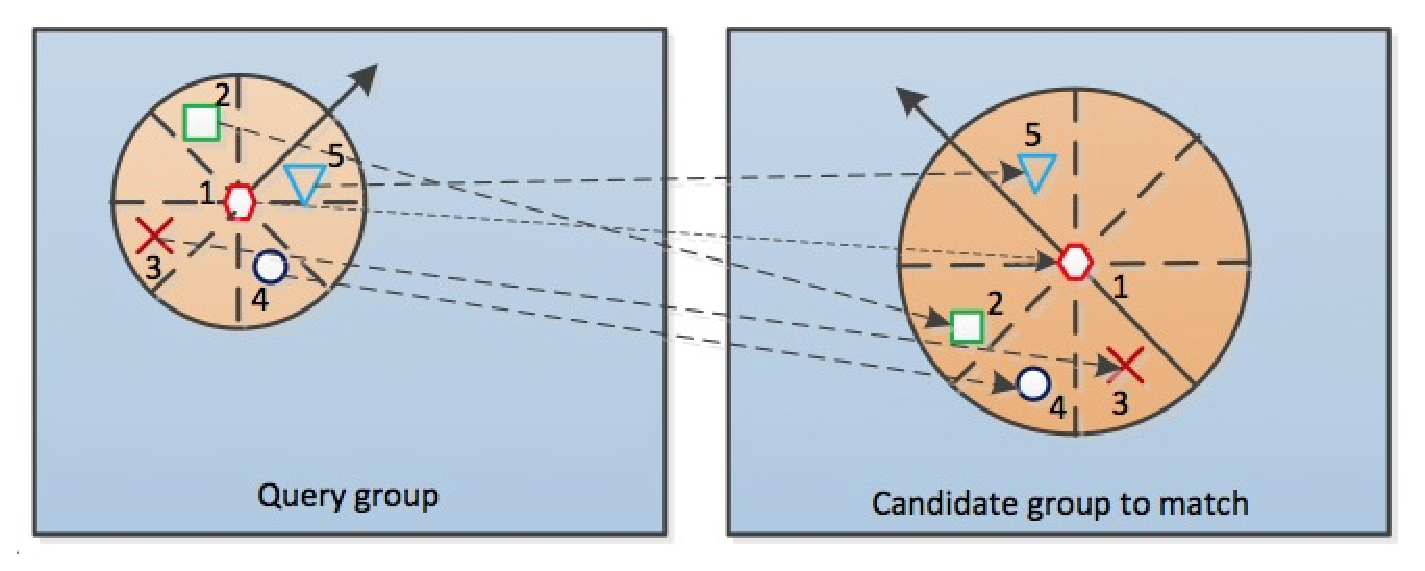
\includegraphics[width=15.00cm]{imgs/ch3/visual_group}
\caption{视觉词组二维编码}
\label{fig:visual_group}
\end{figure}

%-----------------------------------------自己的内容,自适应阈值的图像块筛选法----------------------------------------
\subsection{自适应阈值图像块筛选法}
图像重建任务的最后一个步骤是图像融合,在此之前我们已经得到了每个原图像特征对应的候选图像块,每个图像块有其自身的方向、尺度、位置,图像块之间可能存在交叠。其中有些图像块与原图在像素值上存在较大的出入,需要利用上采样图像计算配准后的图像块与原图像块的误差,根据设定好的阈值\(\epsilon\)移除误差较大的图像块。

原图像经过特征提取、过滤操作后,有几百个大尺度图像块,在分布密集区域,图像块有大量的重叠,并不需要对每一个候选图像块做最后的拼接。利用相似图像搜索得到候选图像,在候选图像中利用特征匹配找到原图像块匹配的候选图像块,虽然在SIFT描述子级别上两个候选图像块是匹配的,但无法保证像素级别上的一致。

在文献\cite{Dai:2012vn}中,使用上采样图像\(I_u\)来校验候选图像块是否正确。校验规则为是

\begin{align}
\label{eq:errorControl}
  \text{Verify}(P_{\tilde{S}}) = 
\begin{cases} 
\text{true}, & \mbox{if MSE} (T(P_{\tilde{S}}),P_c \in I_u) < \epsilon \\
\text{false}, & \mbox{otherwise}
\end{cases}
\end{align}

其中\(\text{MSE}(\cdot,\cdot)\)表示的是两个图像块的均方误差(Mean Square Error)。\(T(P_{\tilde{S}}\)表示对候选图像块进行透视变换,\(P_{S}\)是\(P_{\tilde{S}}\)经过透视变换后在\(I_u\)上的相匹配区域。\(\epsilon\)表示一个阈值常数,当两个图像块的均方误差大于一个阈值时,判定为该图像块匹配失败,否则认为是正确匹配。这里的难点是误差阈值\(\epsilon\)的确定,阈值设定过大,错误匹配块无法筛掉,阈值设定太小,筛选掉相对准确的匹配块,导致最后拼合有缺陷。一般情况下根据经验人为的指定一个相对合理的阈值。

在文献\cite{Dai:2012vn}中提到了对上述配准后的图像块使用基于图的图像分割方案,对每一个分割连通域做均方误差校验,相当于图像块做进一步的细分,能够有效去除图像块中与原图不一致的部分。在实际测试中,我们发现一方面图像分割占用大量的计算资源,这主要是由于我们的重建图像和候选图像分辨率高,而图像分割时间消耗与图像像素数量成正比;另一方面分割导致图像粒度过细,验证步骤的误差存在难以保证筛选结果的准确,因此我们在此省略了精细化分图像块的步骤,提出了一种自适应阈值的图像块筛选法。

我们发现在公式\ref{eq:errorControl}中,因为\(I_u\)是由原始图像经过下采样、编解码、再上采样得到,上采样图像与原始图像在各个区块本身包含了误差,而且误差的大小与每一幅特定的图像以及图像的降采样和插值方式有关。如果我们设定一个固定的阈值,对于有些请求图像来说,可能会筛掉正确的块,对于另一些请求图像,可能会保留错误的匹配块。

针对上述出现的阈值设置的难题,我们设计了一种在客户端完成的阈值自适应的方法,能够根据请求图像的不同动态的调整验证阈值。

实验中我们发现,原始图像高频区域的图像块经过降采样再插值后得到的图像块与原始像素值有了较大的区别,平滑区域图像块经过降采样和插值处理后像素值的整体变化较小,有着较小的误差。又因为原始图像和候选图像在局部区域上往往是角度、透视的变换,在像素值的梯度场的变化两者是一致的,所以原始图像与上采样图像的误差也反映了候选图想与上采样图像之间的误差。

有些原始图像整体较为平滑,与\(I_u\)误差不大,能够较好的反映原图的像素信息,这类使用较低的误差阈值能够得到较好的重建效果,与此相反,有些图像整体或者局部包含大量高频信息,图像\(I_u\)经过了平滑处理在像素信息上有了较大的损失,再使用小的阈值会导致误筛掉正确的匹配块。
自适应阈值方法在客户端计算每一个原始图像块上,计算每一个图像块在上采样图像块和原始图像块上的均方误差,在所有的均方误差数值中选取一个适当的值作为基准误差,再根据服务器端匹配的候选区块数量加上一定的宽容度。

自适应阈值方法的步骤是:
\begin{enumerate}
\item 提取图像\(I\)的SIFT算子,保留其中大于指定尺度的SIFT算子
\item 对原始图像\(I\)进行降采样、编码、解码、上采样,得到\(I_u\)
\item 计算每一个SIFT算子对应的图像块\(P_S\)
\item 计算每一个图像块在\(I\)和\(I_u\)上的均方误差,找到其中最大的作为基准误差\(\epsilon_b\)
\item 在服务器端利用候选相似图像几何做SIFT匹配得到匹配块,根据匹配块的数量M,计算宽容度\(\frac{C}{M}\)
\item 得到最终的验证误差阈值为:
\begin{align}
\epsilon = \epsilon_b + \frac{\epsilon_C}{M}
\end{align}
\end{enumerate}

其中\(\epsilon_C\)为一常数,\(\frac{\epsilon_C}{M}\)的意义是当匹配图像块数量较少时,容许的宽容度增大,尽量保证匹配的图像块能够作为重建图像的一部分,当候选图像块较多时,宽容度变小,重建条件变得苛刻。在步骤四找基准误差时,可以比较最大值与第二大的数值之间的差值,如果过大,说明最大值可能是异常点,可以将其移除后重复步骤四。

%-----------------------------------------结束----------------------------------------

%%%%------------------------------------适用于旅游景点图像的相似图像搜索技术----------------------------------------%%%%
%\section{适用于旅游景点图像的相似图像搜索技术} 可以不提到

%% 本章参考文献
\ifx\usechapbib\empty
\nocite{BSTcontrol}
\bibliographystyle{buptgraduatethesis}
\bibliography{bare_thesis}
\fi